\documentclass[tikz,border=12pt]{standalone}
\usepackage{tikz}
\usetikzlibrary{shapes.geometric,arrows.meta,positioning,fit,backgrounds,calc}

\renewcommand{\familydefault}{\sfdefault}
\definecolor{cborder}{HTML}{1E293B}
\definecolor{cbg}{HTML}{F8FAFC}
\definecolor{cbox}{HTML}{FFFFFF}
\definecolor{cgray}{HTML}{64748B}
\definecolor{cgreen}{HTML}{059669}
\definecolor{cgreenlight}{HTML}{ECFDF5}
\definecolor{cred}{HTML}{DC2626}
\definecolor{credlight}{HTML}{FEF2F2}

\begin{document}
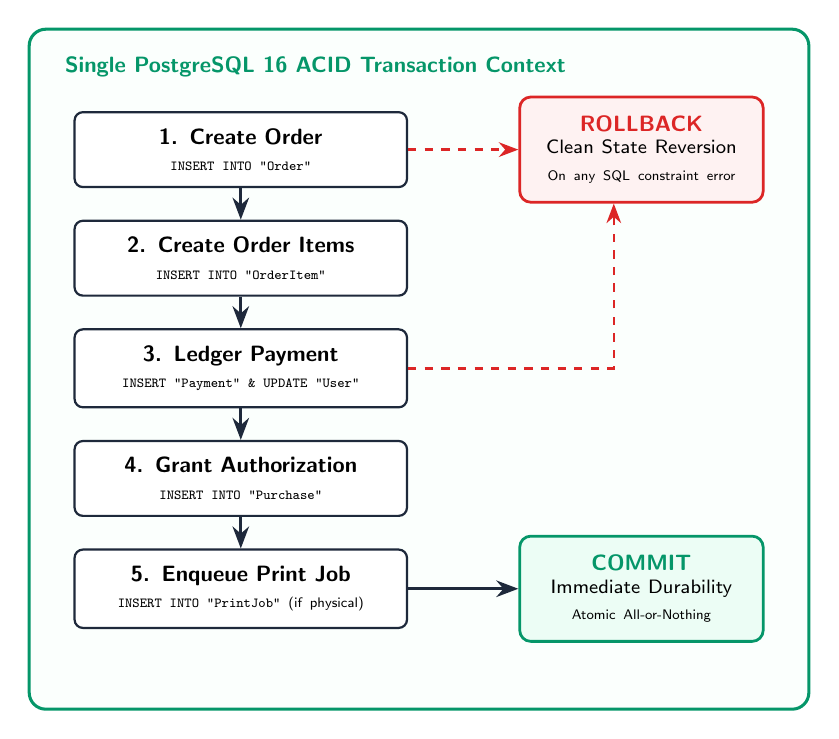
\begin{tikzpicture}[
    font=\small,
    >=Stealth,
    node distance=0.45cm and 1.2cm,
    stepnode/.style={
        draw=cborder,
        fill=white,
        rounded corners=3pt,
        line width=0.8pt,
        align=center,
        inner sep=6pt,
        font=\footnotesize,
        text width=3.8cm
    },
    flow/.style={
        ->,
        line width=1.1pt,
        draw=cborder
    },
    errflow/.style={
        ->,
        line width=0.9pt,
        draw=cred,
        dashed
    }
]

    % Steps placed vertically
    \node[stepnode] (s1) {
        \textbf{1. Create Order}\\
        \tiny \texttt{INSERT INTO "Order"}
    };

    \node[stepnode, below=0.4cm of s1] (s2) {
        \textbf{2. Create Order Items}\\
        \tiny \texttt{INSERT INTO "OrderItem"}
    };

    \node[stepnode, below=0.4cm of s2] (s3) {
        \textbf{3. Ledger Payment}\\
        \tiny \texttt{INSERT "Payment" \& UPDATE "User"}
    };

    \node[stepnode, below=0.4cm of s3] (s4) {
        \textbf{4. Grant Authorization}\\
        \tiny \texttt{INSERT INTO "Purchase"}
    };

    \node[stepnode, below=0.4cm of s4] (s5) {
        \textbf{5. Enqueue Print Job}\\
        \tiny \texttt{INSERT INTO "PrintJob"} (if physical)
    };

    % Outcome nodes on right
    \node[draw=cred, fill=credlight, rounded corners=4pt, line width=1pt,
          right=1.4cm of s1, font=\footnotesize, text width=2.6cm, align=center, inner sep=7pt] (rollback) {
        \textbf{\color{cred} ROLLBACK}\\
        \scriptsize Clean State Reversion\\
        \tiny On any SQL constraint error
    };

    \node[draw=cgreen, fill=cgreenlight, rounded corners=4pt, line width=1pt,
          right=1.4cm of s5, font=\footnotesize, text width=2.6cm, align=center, inner sep=7pt] (commit) {
        \textbf{\color{cgreen} COMMIT}\\
        \scriptsize Immediate Durability\\
        \tiny Atomic All-or-Nothing
    };

    % Connections
    \draw[flow] (s1) -- (s2);
    \draw[flow] (s2) -- (s3);
    \draw[flow] (s3) -- (s4);
    \draw[flow] (s4) -- (s5);

    \draw[flow] (s5) -- (commit);
    \draw[errflow] (s1) -- (rollback);
    \draw[errflow] (s3) -| ([xshift=-10pt]rollback.south);

    % Outer ACID box wrapping all elements with ample padding
    \begin{scope}[on background layer]
        \node[draw=cgreen, fill=cgreenlight!20, rounded corners=6pt, line width=1.1pt,
              fit=(s1) (s5) (rollback) (commit),
              inner xsep=16pt, inner ysep=24pt] (tx_box) {};
    \end{scope}

    \node[anchor=north west, font=\bfseries\footnotesize, text=cgreen] at (tx_box.north west) [xshift=10pt, yshift=-7pt] {
        Single PostgreSQL 16 ACID Transaction Context
    };

\end{tikzpicture}
\end{document}
